\appendix
\chapter{Gantt Chart}
\renewcommand{\thefigure}{A.\arabic{figure}}
\bigskip
\bigskip
\medskip
{\large This section includes the images of the Gantt chart that will represent the timeline for the whole duration of this study.}

\newpage
\begin{figure}[ht]
    \centering
    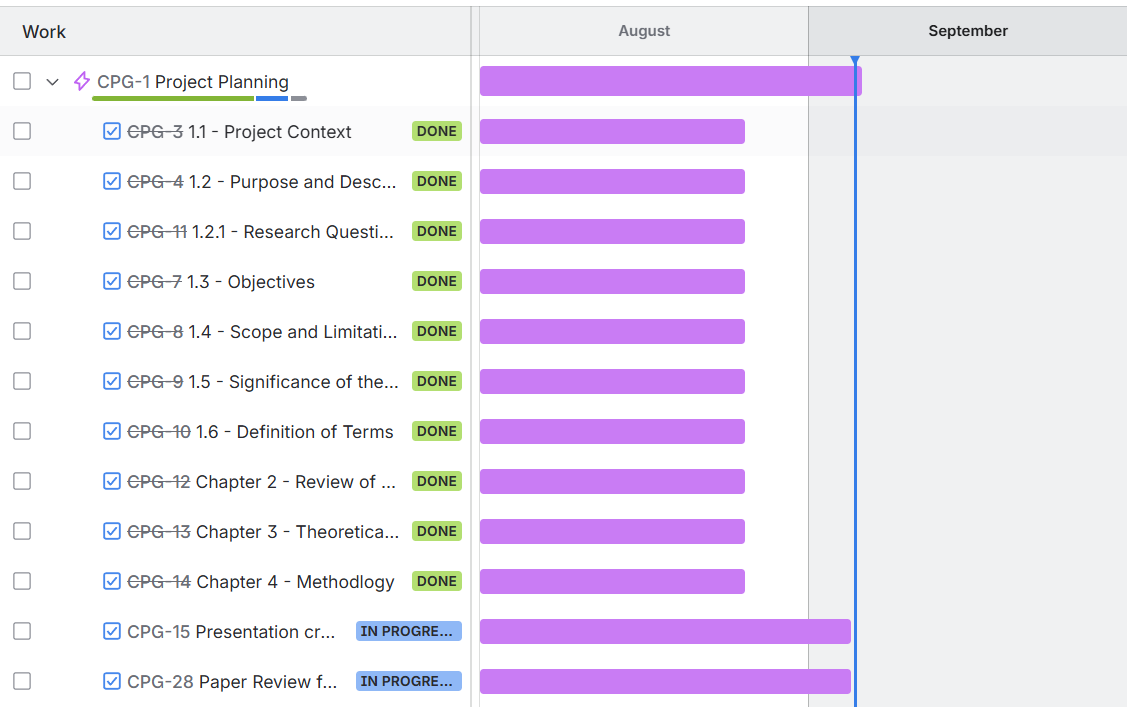
\includegraphics[width=1\textwidth]{figures/aug1-sept5.png}
    \caption{Timeline: August 1 - September 5}
    \label{fig:gantt1}
\end{figure}

\begin{figure}[ht]
    \centering
    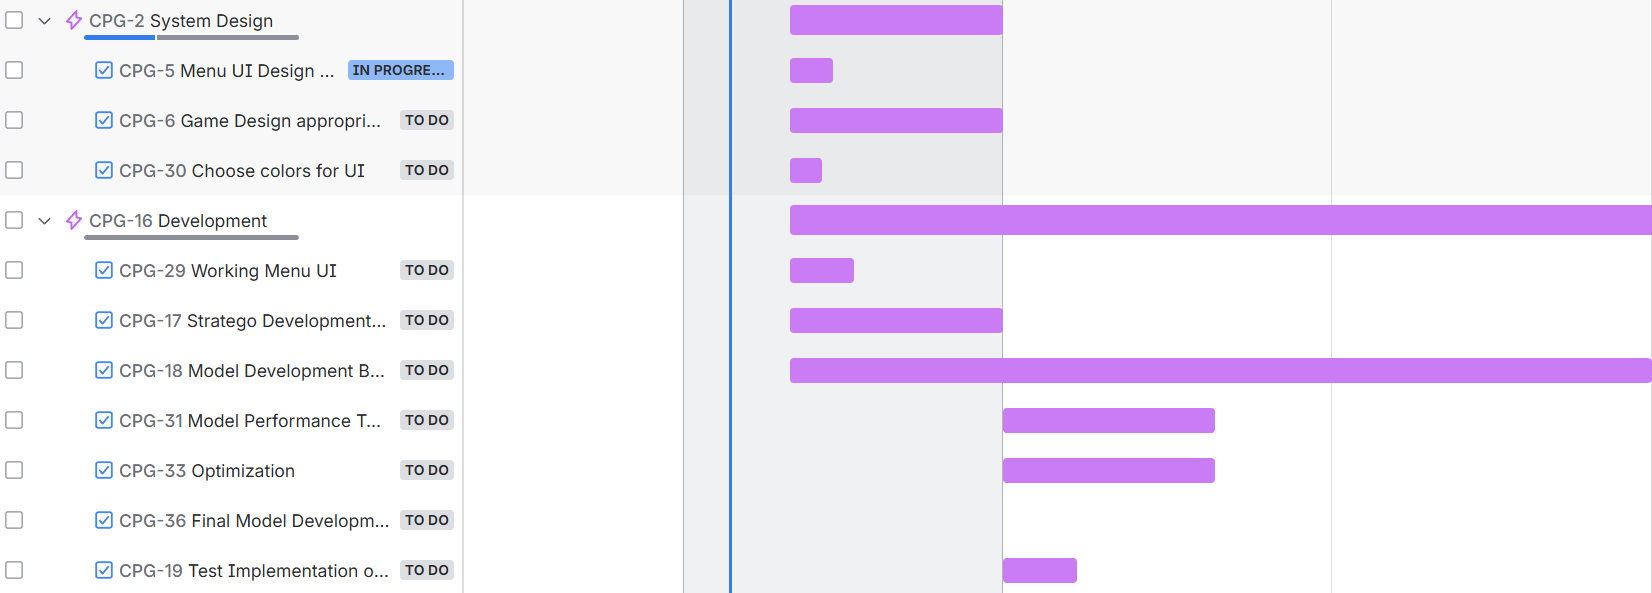
\includegraphics[width=1\textwidth]{figures/sept11-nov30.png}
    \caption{Timeline: September 11 - November 30}
    \label{fig:gantt2}
\end{figure}

\begin{figure}[ht]
    \centering
    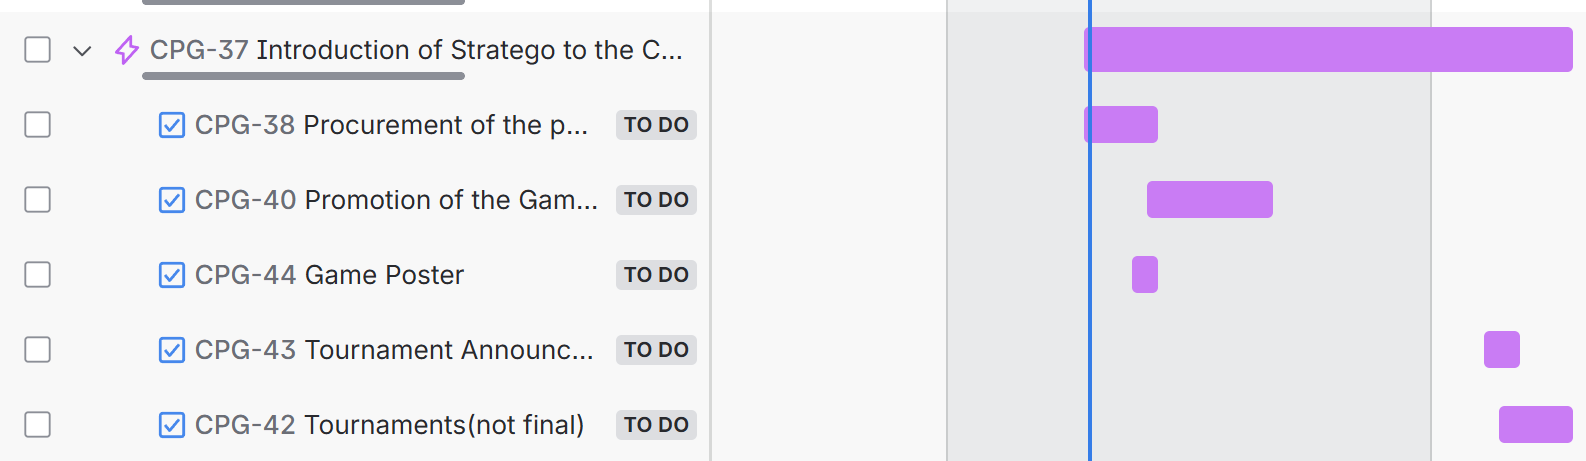
\includegraphics[width=1\textwidth]{figures/oct27.png}
    \caption{Timeline: October 27 - January 27}
    \label{fig:gantt3}
\end{figure}

\begin{figure}[ht]
    \centering
    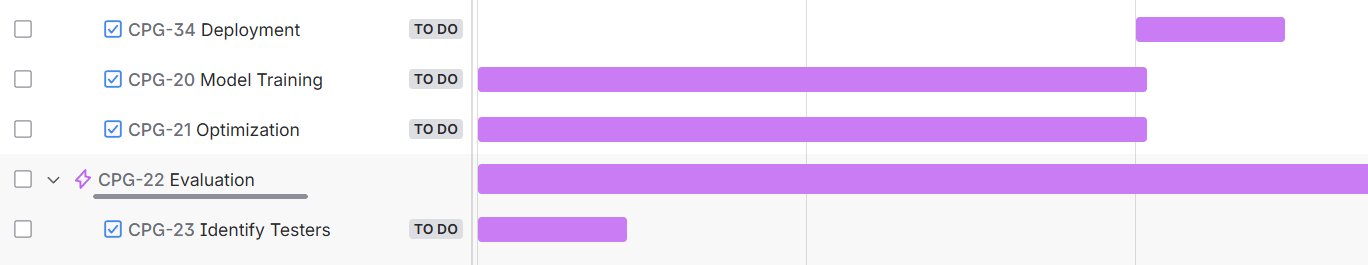
\includegraphics[width=1\textwidth]{figures/dec1-feb14.png}
    \caption{Timeline: December 1 - February 14}
    \label{fig:gantt4}
\end{figure}


\begin{figure}[ht]
    \centering
    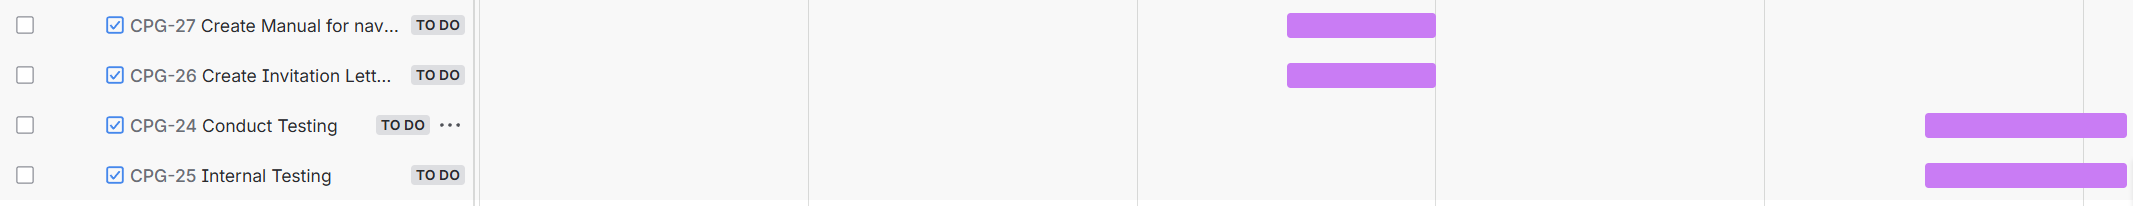
\includegraphics[width=1\textwidth]{figures/feb15-may4.png}
    \caption{Timeline: February 15 - May 4}
    \label{fig:gantt5}
\end{figure}

